\chapter{\IfLanguageName{dutch}{Corpus}{Corpus}}
\label{ch:corpus}

\section{\IfLanguageName{dutch}{Proof of concept}{Proof of concept}}
\label{ch:proof-of-concept}

\subsection{\IfLanguageName{dutch}{Opstelling proof of concept}{Setup proof of concept}}
De uitgewerkte proof of concept (zie figuur:\ref{fig:opstelling_arduino}) is opgesteld uit:
\begin{itemize}
	\item Arduino MKR GSM 1400 Cellular Kit (80.35 euro);
	\item Arduino MKR GPS Shield (41.75 euro);
	\item Lithium Ion Polymeer Accu - 3.7V 2500mAh (25.90 euro).
\end{itemize}
De totale kost van de proof of concept komt neer op \textbf{148.00 euro}. Naast de lage kost heeft de proof of concept de mogelijkheid om zelf volledig geconfigureerd te worden. De configuratie is gebeurd in de editor van Arduino zelf. Het script is in staat om de volgende functies uit te voeren:
\begin{itemize}
	\item De locatie bepalen aan de hand van GPS;
	\item De locatie bepalen aan de hand van GPRS;
	\item De locatie doorsturen naar een REST API aan de hand van een POST request (JSON).
\end{itemize}
Het script is nieuw ontwikkeld en staat opensource op \href{https://github.com/IndyVC/bap-arduino}{een github repository}. In het script werd gebruik gemaakt van verscheidene libraries om het traceren mogelijk te maken.
Er werd gebruik gemaakt van:
\begin{itemize}
	\item \href{https://github.com/arduino-libraries/ArduinoHttpClient}{ArduinoHttpClient}: voor het versturen van data aan de hand van POST requests;
	\item \href{https://github.com/arduino-libraries/MKRGSM}{MKRGSM}: voor het gebruik van mobiele data;
	\item \href{https://github.com/bblanchon/ArduinoJson}{ArduinoJson}: het mogelijk maken om makkelijk een JSON body op te vullen;
	\item \href{https://github.com/arduino-libraries/Arduino_MKRGPS}{ArduinoMKRGPS}: voor het bepalen van de locatie via GPS.
\end{itemize}
De proof of concept maakt gebruik van een simkaart (zie figuur: \ref{fig:simkaart}) om online data te kunnen versturen. 
\begin{figure}
	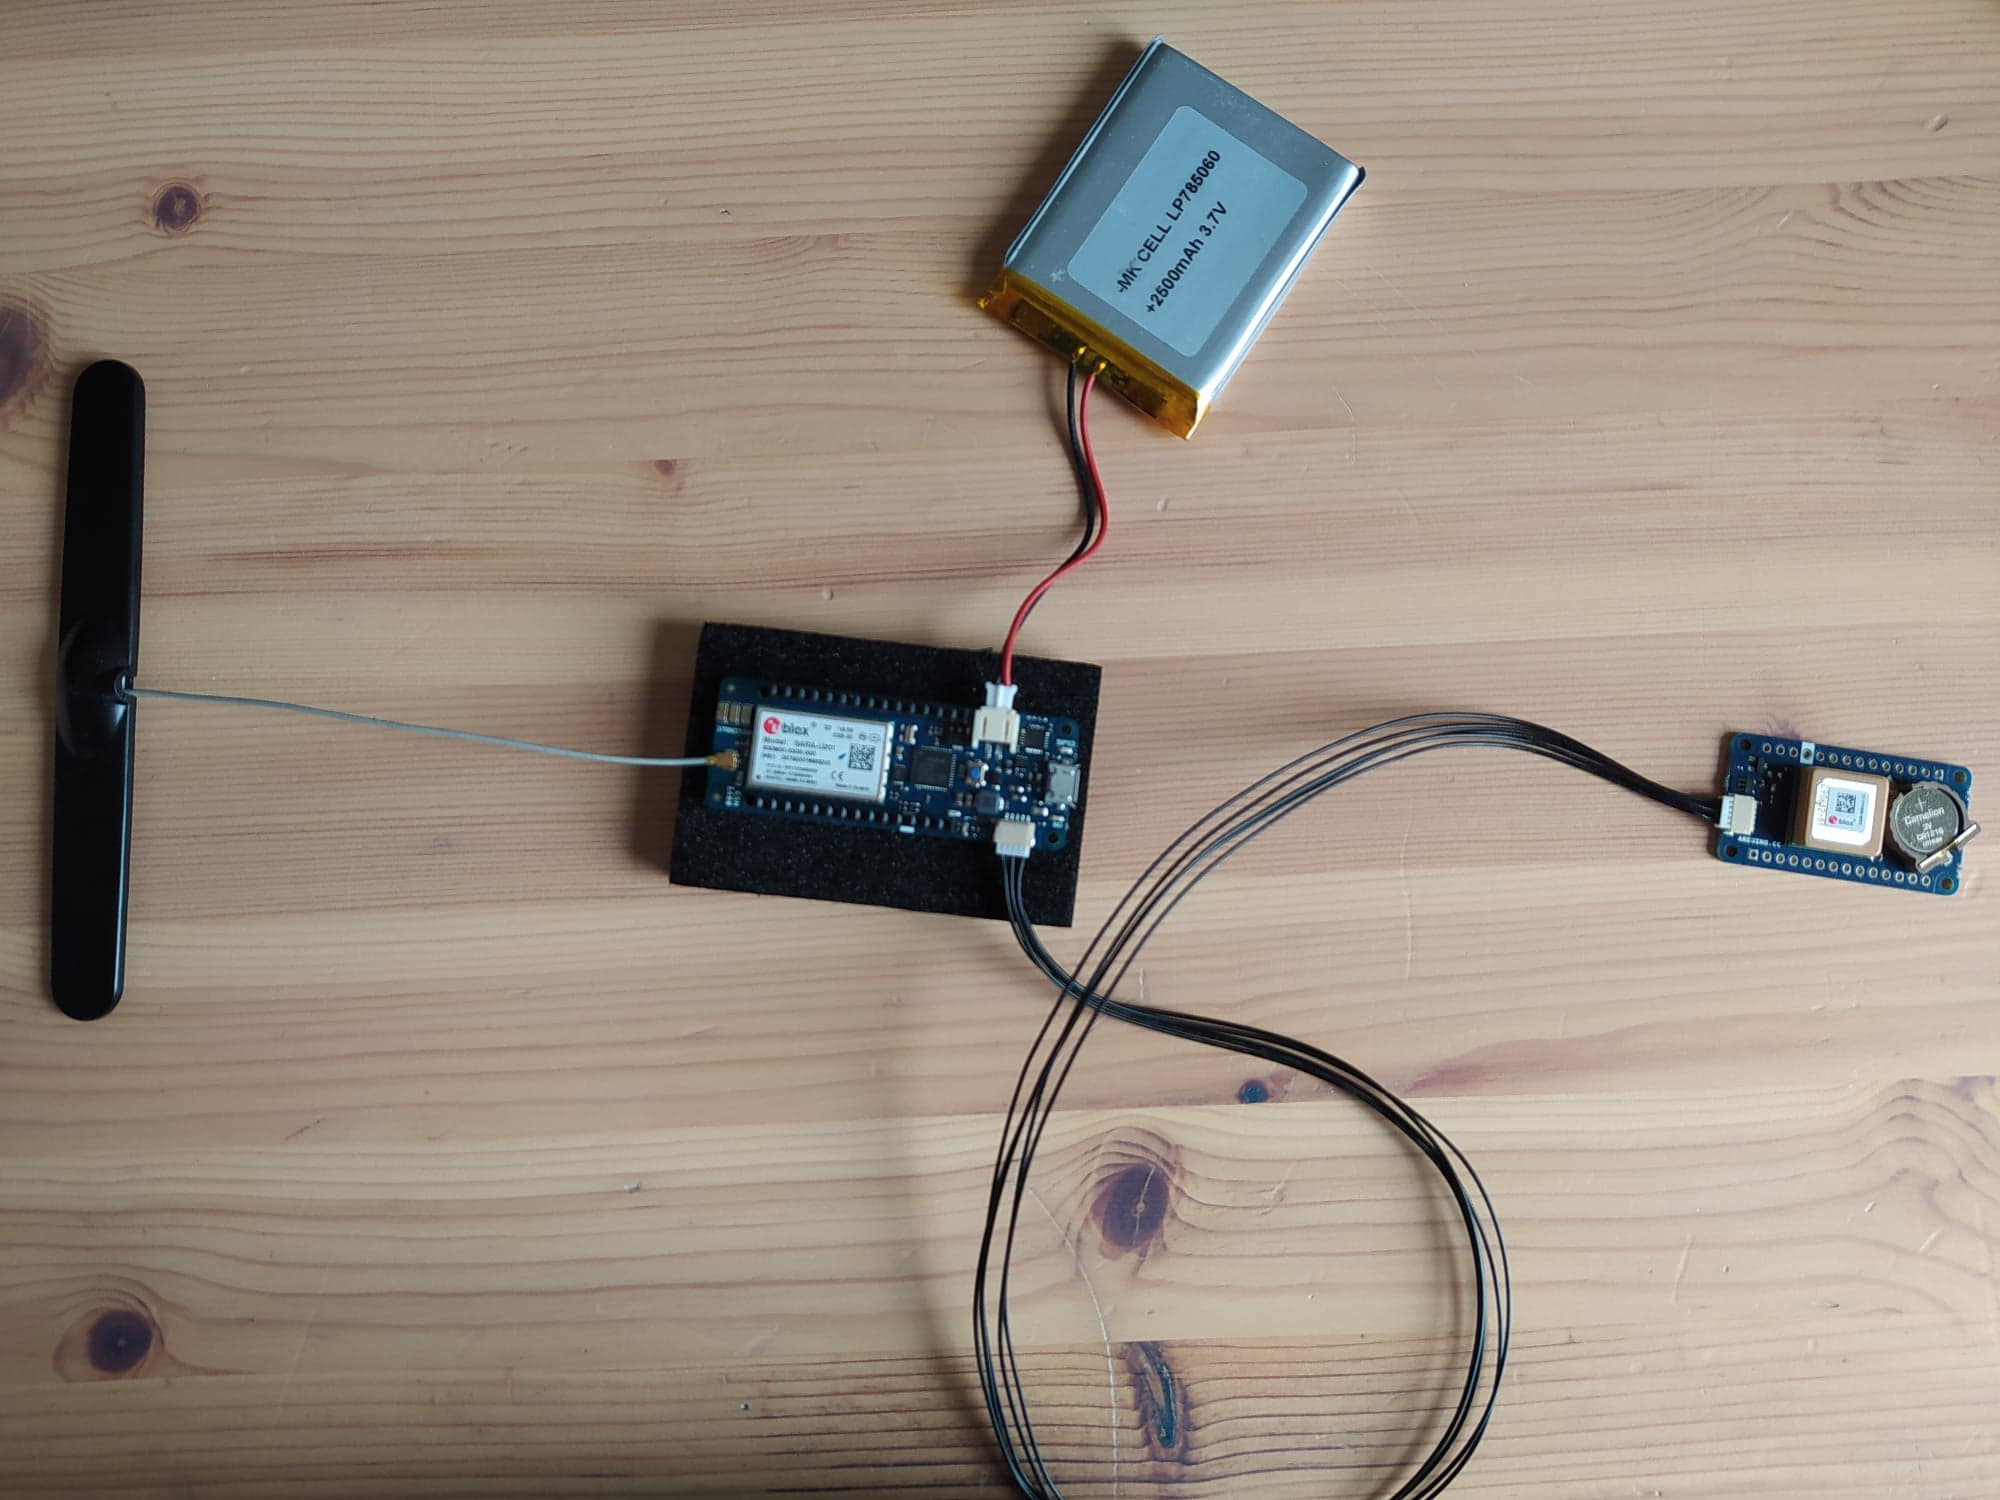
\includegraphics[width=\textwidth,height=\textheight,keepaspectratio]{opstelling_arduino.jpg}
	\caption{opstelling proof of concept}
	\label{fig:opstelling_arduino}
\end{figure}
\begin{figure}
	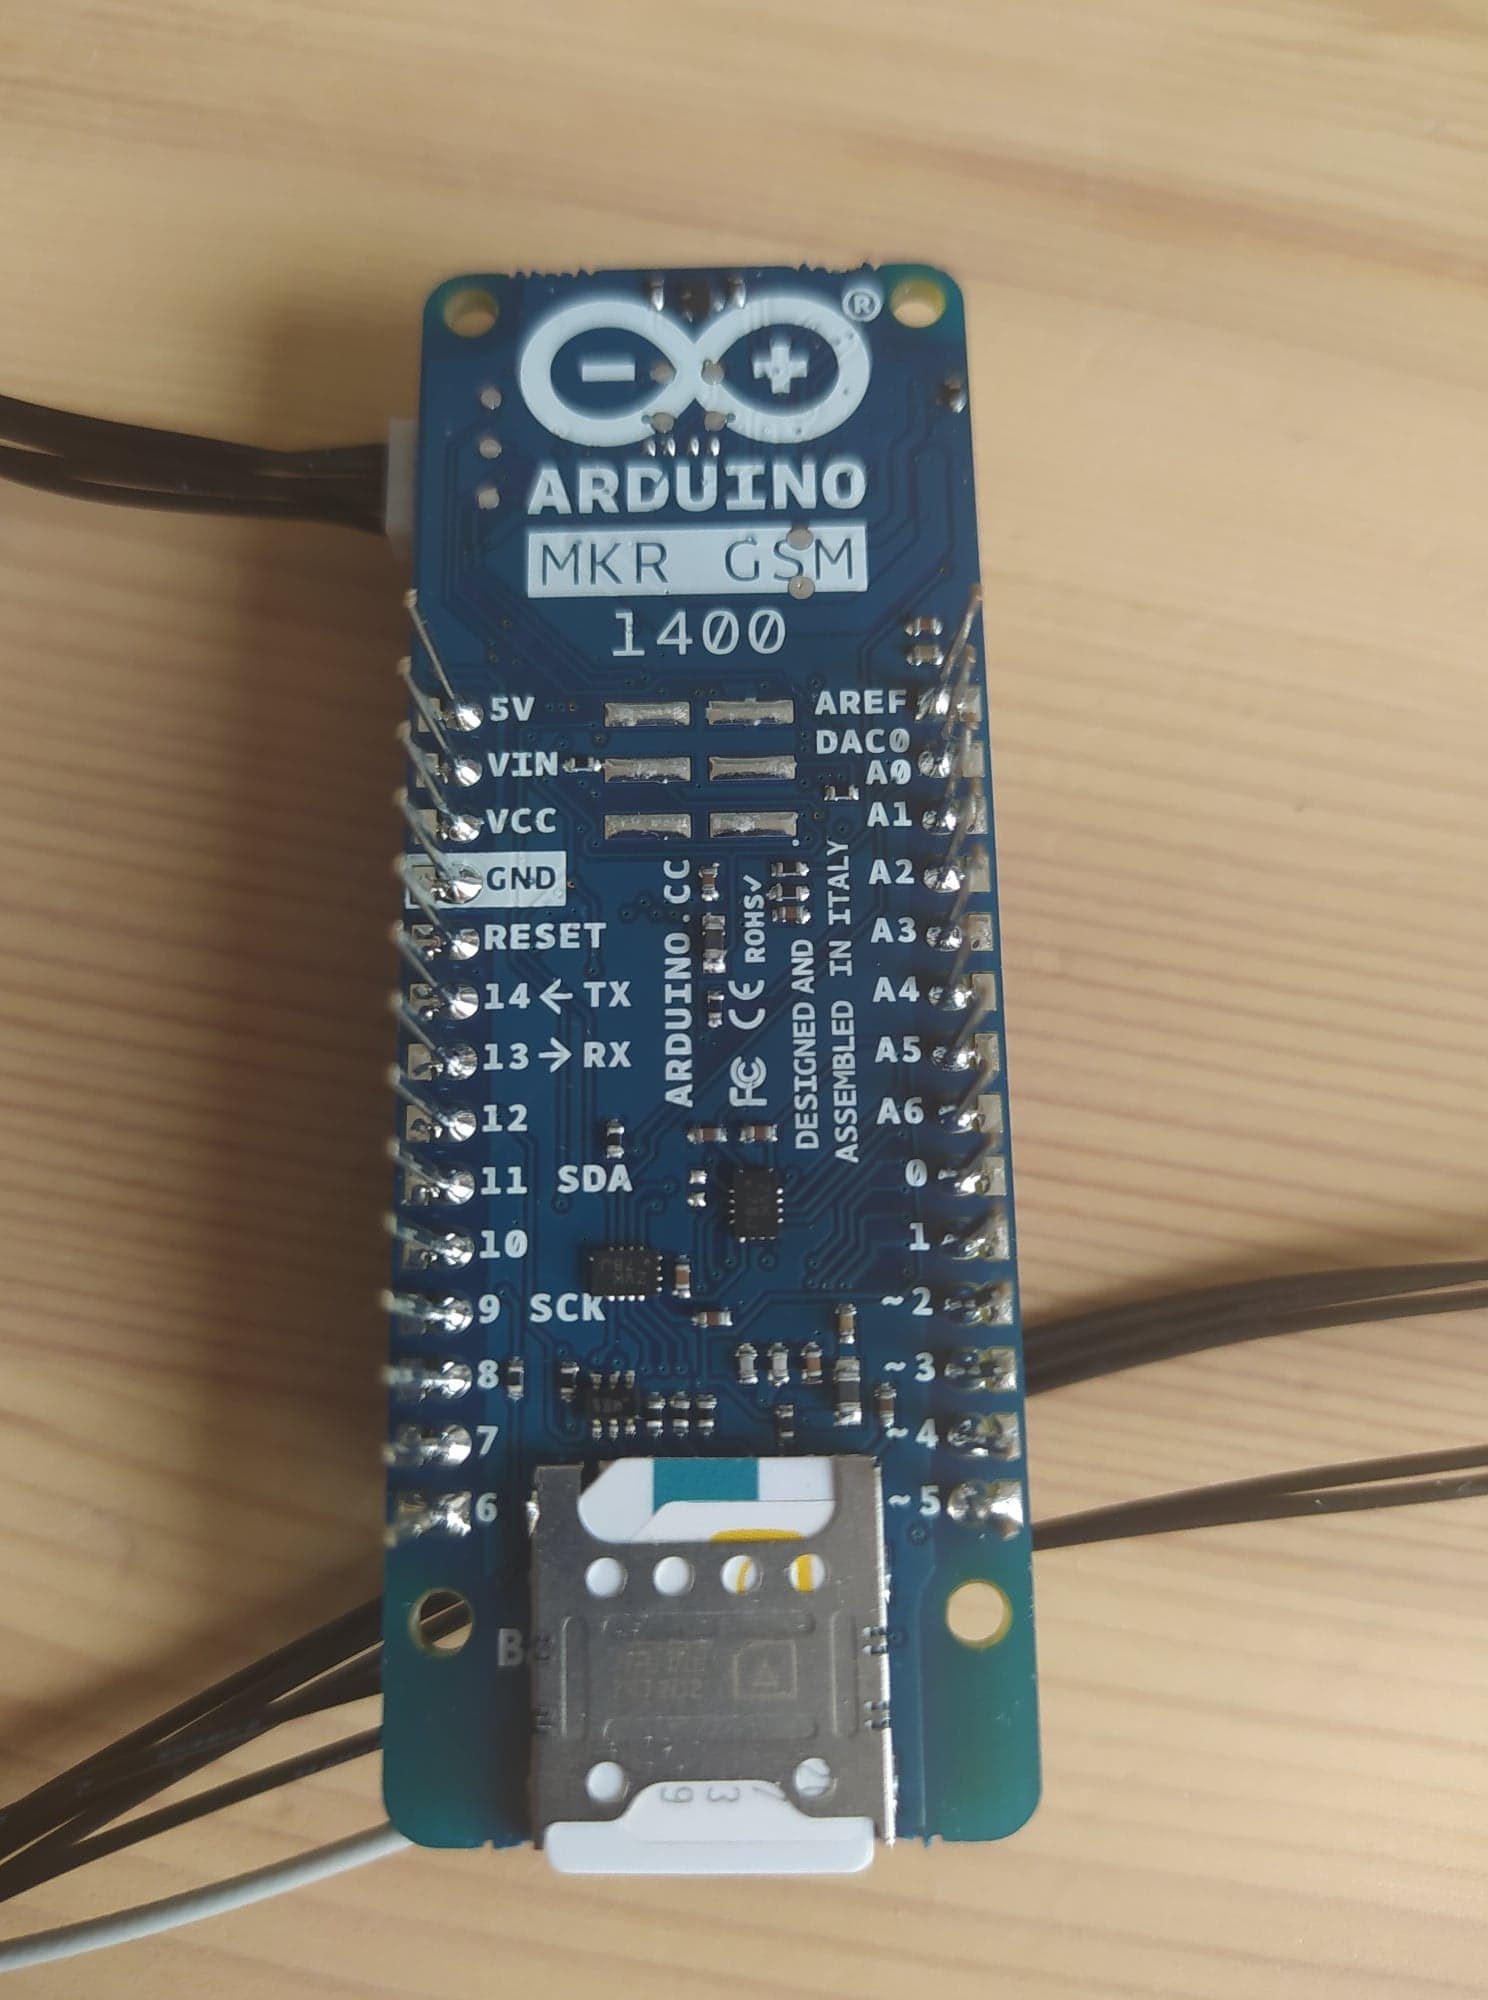
\includegraphics[width=\textwidth,height=\textheight,keepaspectratio]{simkaart.jpg}
	\caption{Simkaart}
	\label{fig:simkaart}
\end{figure}

\subsection{\IfLanguageName{dutch}{Waterdichte casing}{Waterproof casing}}
TODO: NOG AAN TE VULLEN
\pagebreak
\section{\IfLanguageName{dutch}{Backend}{Backend}}
\label{ch:backend}

\subsection{\IfLanguageName{dutch}{Ontwikkeling}{Development}}
Voor backend is er gebruik gemaakt van \href{https://mongoosejs.com/}{Mongoose}. De gehele infrastructuur is gebaseerd op de MEVN stack.
Deze stack staat voor:
\begin{itemize}
	\item Mongoose
	\item Express
	\item Vue
	\item Node.JS
\end{itemize}
Mongoose maakt gebruik van \href{https://www.mongodb.com/cloud/atlas}{MongoDB Atlas}. De backend, geschreven in Javascript, is opensource en staat online op \href{https://github.com/IndyVC/bap-backend}{een github repository}.
\newline
De functie van de backend is het ontvangen van locaties van de proof of concept. Deze locaties worden opgeslagen in een NO-SQL database en houdt de volgende informatie bij per locatie:
\begin{itemize}
	\item longitude
	\item latitude
	\item altitude
	\item snelheid (in km/h)
	\item aantal satellieten
	\item method (locatie bepaalt via GPS of GPRS)
\end{itemize}
De methode hangt af van de beschikbaarheid van het signaal. Indien er geen GPS-signaal gevonden kan worden, schakelt de proof of concept vanzelf over op GPRS. Maar GPS blijft wel de eerste keus omdat dit accurater is dan GPRS. Indien de lokatie bepaalt is via GPRS, zullen de velden snelheid en aantal satellieten leeg zijn. Dit komt doordat GPRS data van gsm-masten gebruikt (zie hoofdstuk \ref{ch:stand-van-zaken}). De lokatie wordt dan niet bepaald door satellieten, maar baseerd zicht op data van gsm-masten. 

\subsection{\IfLanguageName{dutch}{Deployment}{Deployment}}
Naast de code staat ook het programma online. De backend kan \href{https://indy-bap-backend.herokuapp.com/api/locations}{\underline{hier}} bekeken worden. Voor de deployment is er gebruik gemaakt van \href{www.heroku.com}{heroku}. Doordat het programma online draait, kan de \href{https://indy-bap-frontend.netlify.com/}{webapplicatie} deze data ophalen en weergeven.
\newline
Er is echter een nadeel, de backend maakt gebruik van een gratis hosting plan. Hierdoor kan het programma 'slapen' na dertig minuten inactiviteit. Dit wilt zeggen dat u de webapplicatie twee keer moet laden. Een eerste keer om de backend wakker te schudden en een tweede keer om de webapplicatie te gebruiken.
\pagebreak
\section{\IfLanguageName{dutch}{Frontend}{Frontend}}
\label{ch:frontend}

\subsection{\IfLanguageName{dutch}{Ontwikkeling}{Development}}
Zoals reeds verteld is er gebruik gemaakt van de MEVN stack. Dit wilt zeggen dat de webapplicatie ontwikkeld is in Vue, een nieuwer javascript-framework. De code van deze webapplicatie is opensource en staat online op \href{https://github.com/IndyVC/bap-frontend}{een github repository}.
\newline
Voor de webapplicatie (zie figuur: \ref{fig:webapplicatie}) is er gebruik gemaakt van 'google maps'. Google maps is een veelgebruikte technologie waardoor dezelfde layout een vorm van betrouwbaarheid en herkenbaarheid geeft. Hierdoor voelt de webapplicatie gemakkelijk aan om te gebruiken. Naast het tracken zelf, weergeeft het ook extra informatie, zoals welke methode gebruikt wordt, hoe snel de GPS-tracker zich voort beweegt en hoe betrouwbaar de coördinaten zijn (aantal satellieten). De gebruiker is instaat om de geschiedenis van lokaties te verwijderen aan de hand van een knop.
\newline
Voor de implementatie van google maps is er gebruik gemaakt van een opensource en gratis te gebruiken library, namelijk \href{https://www.npmjs.com/package/vue2-google-maps}{vue2-google-maps}.
\begin{figure}
	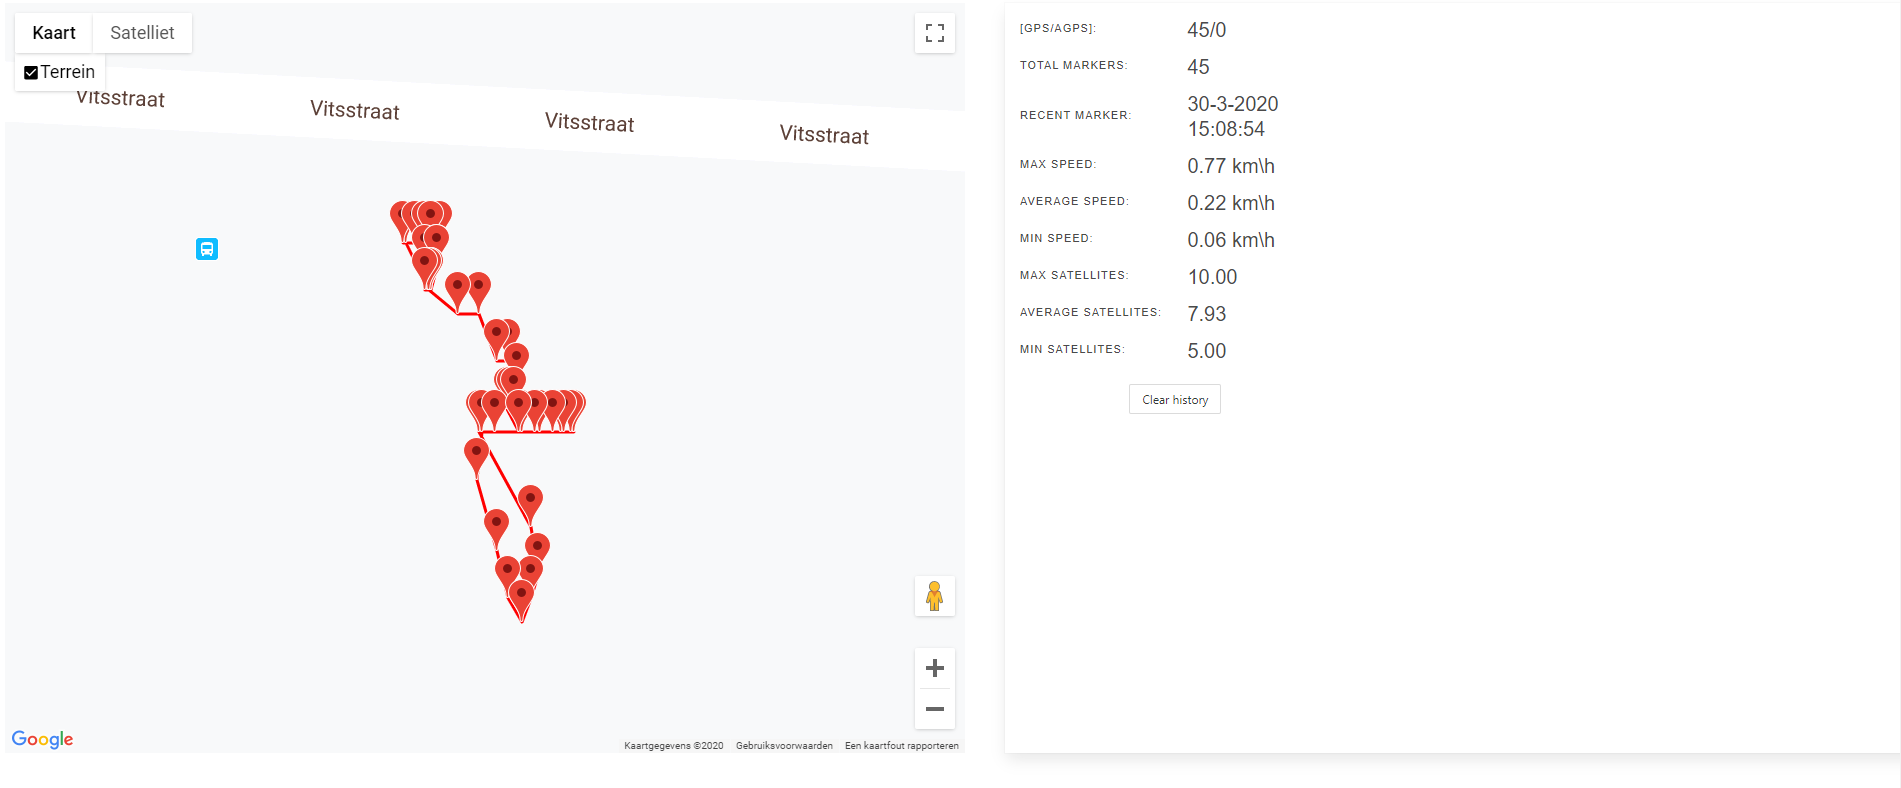
\includegraphics[width=\textwidth,height=\textheight,keepaspectratio]{webapplicatie.png}
	\caption{Webapplicatie}
	\label{fig:webapplicatie}
\end{figure}

\subsection{\IfLanguageName{dutch}{Deployment}{Deployment}}
Voor de website online te zetten is er gebruik gemaakt van netlify. \href{https://www.netlify.com/}{Netlify} is een hosting bedrijf dat een gratis plan aanbiedt. De webapplicatie staat \href{https://indy-bap-frontend.netlify.com/}{\underline{hier}} online.